\documentclass[../../main.tex]{subfiles}


\begin{document}

    The software for NA62 is split into three main \sloppy\texttt{C++} packages: NA62MC, NA62Reconstruction and NA62Analysis. NA62MC is a GEANT4 based Monte Carlo simulation package that simulates the NA62 experiemnt including the detector geomtery and the full simulation of 
    kaon decays, used as a comparison to the data collected by the experiment. NA62Reconstruction is a package that is used to reconstruct either the Monte Carlo data or collected data from the experiment for all detectors. NA62Analysis is used by the physicists to analyse the data produced from the reconstruction to 
    produce all the physics studies that are conducted at NA62. 

    The NA62 software was designed for use only with the NA62 experiment resulting in in minimal configurability and flexibility, with the only option for users to change the software being to enable/disable sub-detectors. With the experiment forseen to run up to CERNs Long shutdown 3 (LS3), an upgraded software package was needed to allow
    for the development of new detectors for the future kaon experiments. This software had to be flexible and configurable to allow for the simulatinous use of the software for NA62 data taking and physics analysis, as well as the development of new experiements.
    \section{FlexibleMC}
    \subsection{Description}
    For the implementation of a flexible framework all detector classes were refactored to inherit from a common class which contianed the basic functions and variables for all detectors allowing for all classes to be parsed using the same machinery. The input to the simulation was then changed to allow for the configuration of all the detectors to be read in from a configuration file which contained any varibles required for individual detectors and the X,Y,Z and rotation of the detectors. 
    An example entry in the configuration file is shown in Figure \ref{fig:config} where a name was given for the station "STRAW0", along with chamber ID, chmaber type which defines the size of the straws and the chamber geometry which defines if the beam hole is symetric or not. The varibles for each subdetector are defined in Table  

    \begin{figure}[H]
        \centering
        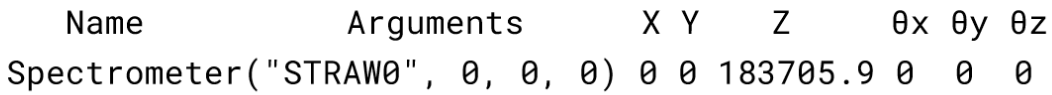
\includegraphics[width=0.8\textwidth]{imgs/example_config.png}
        \caption{Example configuration for the STRAW0}
        \label{fig:config}
    \end{figure}

    \begin{table}[H]
        \centering
        \begin{tabular}{|l|l|}
        \hline
        Detector Name & Variables \\ \hline
        STRAW & \begin{tabular}[c]{@{}l@{}}Chamber ID: 0,1,2,3\\ Chamber Type:  0(10mm), 1(5mm) \\ Chamber Mode: 0(default), 1(symmetric)\end{tabular} \\ \hline
        Spectrometer Magnet & Magnetic field intensity \\ \hline
        Vessel & \begin{tabular}[c]{@{}l@{}}Length\\ InnerRadius\\ OuterRadius\\ Type("BlueTube", "BlueTubeNoRails", "GreyTube")\end{tabular} \\ \hline
        \end{tabular}
        \caption{}
        \label{tab:config_variables}
    \end{table}

    When built inside the simulation, each detector was now contained within its own separate volume called the "Responsibility Region". This was a simple task for most detectors apart from the STRAWs and LAV which were made up of multiple stations that were not continuous, resulting in multiple responsibility regions for each station.

    \subsection{Testing: Geometry and Magnetic Fields}
    After the simulation was upgraded all the geometries of each detector had to be validated that they were still correct with respect to the previous version. This was due to the complex nature of refactoring the detectors and that a number volumes had been changed. The validation was completed using the GEANT4 , which is a virtual particle present in the simulation package that will travel in a straight line and interact with all volumes 
    present in the simulation. It was then possible to produce a large square beam of these particles and save every time the particle passed though a boundary between two volumes. Using this it was possible to check the placement and geometry of each detector to mm precision to ensure that the simulation was still accurate. An example of the geantino hits on a single view of STRAW chamber 1 is shown in Figure \ref{fig:geantino_plot} where 
    it is possible to see the features of the view. For the full validation a larger sample of Geantinos is used to get the required precision, however when there was a discrepancy they were sent in a much smaller area.

    \begin{figure}[H]
        \centering
        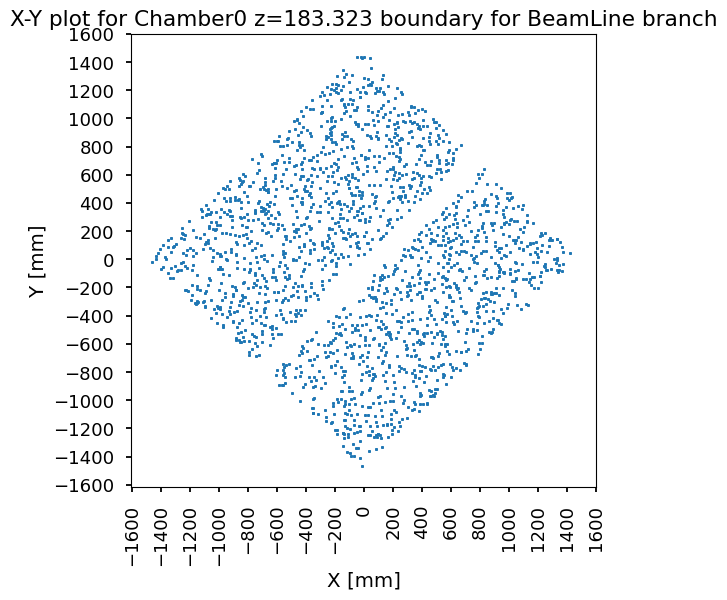
\includegraphics[width=0.6\textwidth]{plots/XY_CHBR0_Beam.png}
        \caption{Geantino hits on a single view in straw chamber 1}%
        \label{fig:geantino_plot}%
    \end{figure} 

    To reduce the chance of overlaps and to clean up the simulation, a campaign to reduce the size of the unused space in all sub-detectors. The outer volume (Responsibility Region) for all detectors were reduced to just slightly larger than the physical detector which is possible to see in figure \ref{fig:fields}, as the magnetic fields are calculated in the all volumes not the world volume. In \ref{fig:fields}(a) the field was calculated outside of the 
    actual physical sub-detector due to the larger outer volume, whereas in \ref{fig:fields}(b) the volume has been reduced to a few mm's bigger than the actual physical detector and as a result the field is calculated in the correct region.

    To improve the usability for users a geometry check is completed every time before the simulation is ran. Each outer detector volume is checked for any overlaps with other detectors in all three dimensions taking into account any rotations and the shape of the outer volumes, if a overlap is found the simulation does not start and an error is produced to the user describing where the overlap is and what detectors are involved. 

    \begin{figure}[H]
        \begin{minipage}{\linewidth}
            \centering
            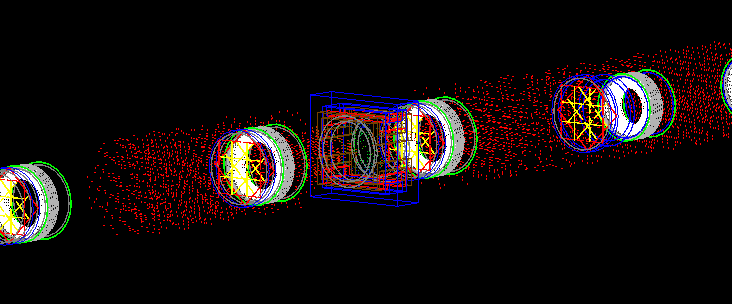
\includegraphics[width=\linewidth]{imgs/old_mag.png}
            \vspace{0.5em} % Adds space between the image and the caption
            \makebox[\linewidth]{\small (a) Previous NA62MC Magnetic field calculations}
    
            \medskip
    
            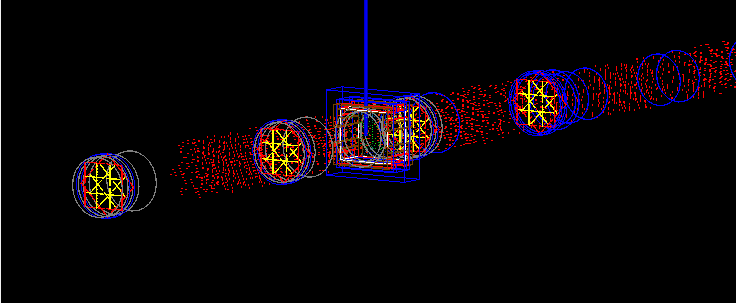
\includegraphics[width=\linewidth]{imgs/new_mag.png}
            \vspace{0.5em} % Adds space between the image and the caption
            \makebox[\linewidth]{\small (b) Upgraded NA62MC Magnetic field calculations}
        \end{minipage}
        \caption{Visualisation from NA62MC of the magnetic field in the spectrometer region}
        \label{fig:fields}
    \end{figure}

    The magnetic field in the simulation is based of real-world measurements of the magnetic field at NA62 from hall probes \cite{Fry_2016}, with this information saved in the form of data files which is taken in and used to calculate the magnetic field at various points in the simulation. In NA62MC the magnetic field is split into three distinct regions; Bluetube which is the magnetic field within the decay region which is used for small corrections, 
    fringe field which are the edges of the MNP33 magnetic field and the MNP33 field which is the main magnetic field defined in the simulation from the MNP33 magnet. In the previous version of the simulation the position of the magnetic fields were hard coded, however in the upgraded version it was possible to move the MNP33 magnet to be placed in any position, requiring the  magnetic field to be calculated relative from that position.  An example of this flexibility is shown in Figure \ref{fig:moved_mag} where 
    the MNP33 magnet was moved from 198\,m to 163\,m in front of the straw chamber 1 and the magnetic field was recalculated from that point within the constructed volumes.

    \begin{figure}[H]
        \centering
        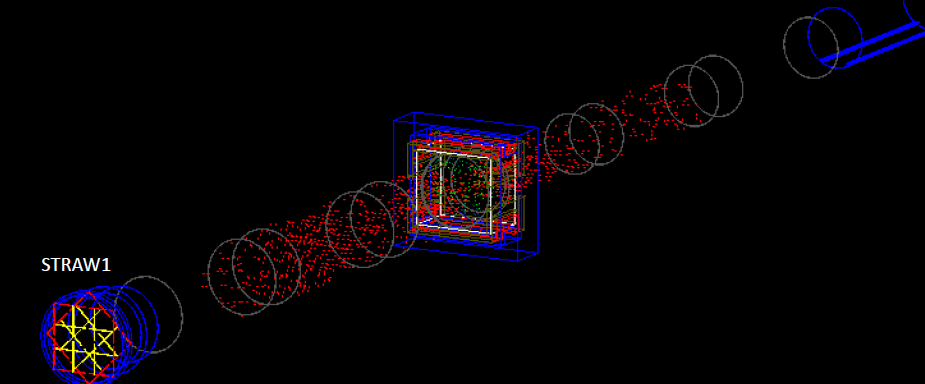
\includegraphics[width=\textwidth]{imgs/move_mag.png}
        \caption{Visualisation from NA62MC with the MNP33 magnet moved in front of the straw chamber 1}%
        \label{fig:moved_mag}%
    \end{figure} 

    The modification of the magnetic fields required validation, which was done using similar machinery to the geometry test completed above but with different GEANT particle, the charged Geantino. Similar to a normal Geantino, but they interact with magnetic fields allowing to ensure that the same tracks were being produced by the new version of the software. An example of this is shown in Figure \ref{fig:mag_check} where it is possible to see the displacement 
    of the charged Geantinos within the field regions. The exact XY positions of the hits would then be validated against a sample of charged Geantinos with the exact mass, momentum and direction produced with the previous version of the software.

    \begin{figure}[H]
        \centering
        \includegraphics[width=\textwidth]{plots/All_xz.png}
        \caption{Charged Geantino hits on all detectors ADD EXTENT OF THE FIELD REGIONS}%
        \label{fig:mag_check}%
    \end{figure} 

    With minimal modification it was also possible to add the functionality to add multiple magnets in the simulation with their magnet fields producing a combined field. This was not implemented into the framework as its use was not foreseen but the machinery was developed and is ready for uses when required. 

    After the geometry and magnetic field tests were completed, full test productions of $K^+ \to \pi^+ \pi0$,  $K^+ \to \pi^+ \pi^- \pi^+$ and $K^+ \to \mu^+ \bar{\nu}$ were produced to test the validity of the existing NA62 setup along with the entire software chain (MC->Reconstruction->Analysis). 
    
    \subsection{Testing: Symmetric NA62}
    It was also required to test the entire software chain using the new features of the flexible framework to ensure that when it was required and used in the future there were no issues. 
    It was proposed to conduct a small study to investigate the feasibilty of a symmetric NA62.

    As described previously in Chapter \ref{sec:na62} the current NA62 detector setup has been optimised for the search of $K^+ \to \pi^+ \nu \bar\nu$ with the current experiement set to run until CERNS LS3. After LS3 it was foreseen that there would be the possiblilty of both charged and neutral kaon experiemnts located at CERN 
    requiring a redesign of the NA62 detector setup. In the current NA62 setup, the beam is deflected in the positive x-direction by the TRIM5 magnet, which is located between GTK stations 2 and 3. The TRIM5 has a strength of $-0.3\,Tm$, which equates to a 90\,MeV kick, deflecting the beam to a maximum deflection of approximately +114\,mm at straw chamber 2. 
    After chamber 2, the MNP33 dipole magnet deflects the beam in the negative x direction with a momentum kick of 270\,MeV. This requires the beam holes for the four Straw stations to be offset from the centre axis as shown in Figure \ref{fig:na62nominal} to allow for the undecayed charged beam to through the spectrometer. The mean beam centre of a charged Kaon at $75\,GeV$ is shown by the red line starting from straw chamber 1 all the way to the LKr accounting for the interactions with the TRIM5 and the MNP33 magnets. 

    \begin{figure}[H]
        \centering
        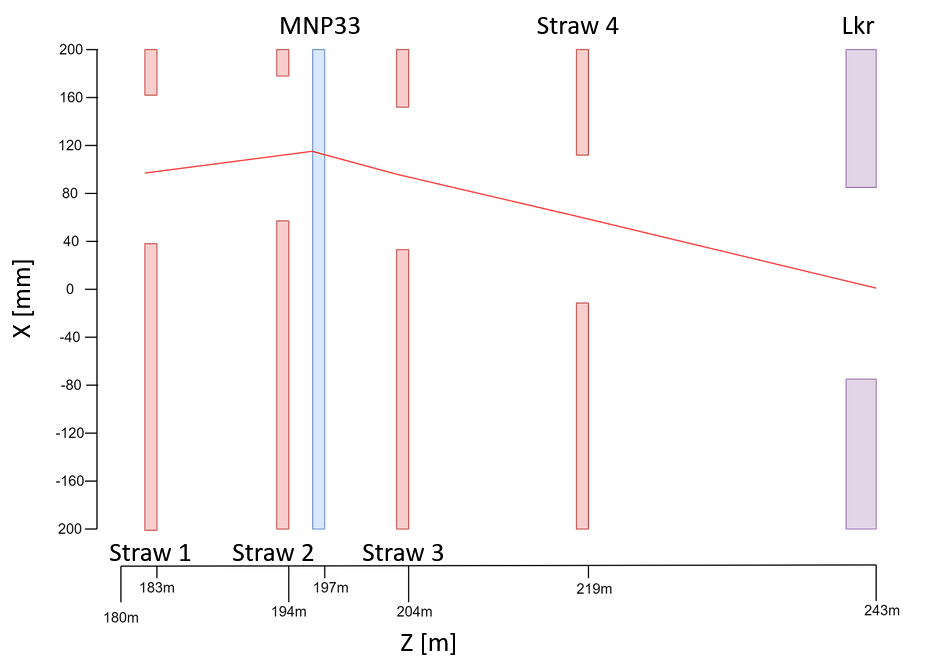
\includegraphics[width=10cm]{imgs/Nomina_diag.png}
        \caption{Diagram showing the path of the charged kaon beam, the straw chamber beam holes and the LKr beam pipe }
        \label{fig:na62nominal}
    \end{figure}

    The exact positions of the NA62 straw chambers and the beam holes are defined in Table \ref{tab:strawcharc}.
    \begin{table}[H]
        \centering
        \begin{tabular}{|c|c|c|}
        \hline
        Straw Chamber & \begin{tabular}[c]{@{}c@{}}Z BackFace \\ {[}m{]}\end{tabular} & \begin{tabular}[c]{@{}c@{}}X Hole Displacement\\ {[}mm{]}\end{tabular} \\ \hline
        1 & 183.7 & 101.2 \\ \hline
        2 & 194.26 & 114.4 \\ \hline
        3 & 204.64 & 92.4 \\ \hline
        4 & 219.07 & 52.8 \\ \hline
        \end{tabular}
        \caption{Straw chamber beam hole properties for NA62 detector setup}
        \label{tab:strawcharc}
    \end{table}

    The beam profile at each Straw station is shown in Figure \ref{fig:nombeam}.

    \begin{figure}[H]
        \begin{minipage}{\linewidth}
            \makebox[.5\linewidth]{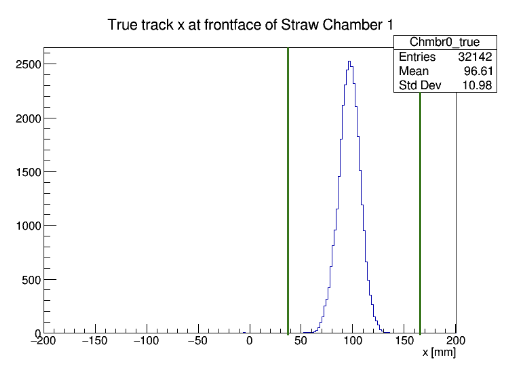
\includegraphics[width=.45\linewidth]{plots/BeamC1.png}}%
            \makebox[.5\linewidth]{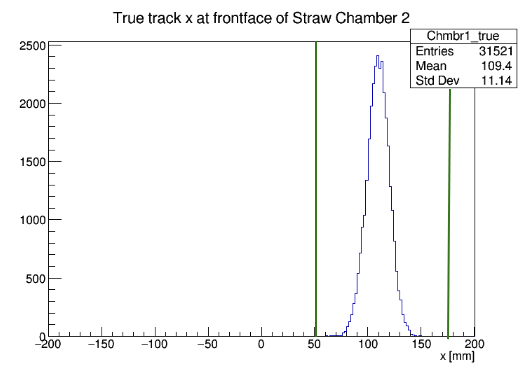
\includegraphics[width=.45\linewidth]{plots/BeamC2.png}}

            \makebox[.5\linewidth]{\small (a) Straw chamber 1}%
            \makebox[.5\linewidth]{\small (b) Straw chamber 2}%

            \medskip

            \makebox[.5\linewidth]{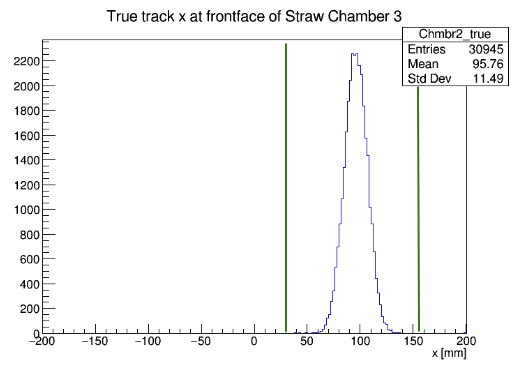
\includegraphics[width=.45\linewidth]{plots/BeamC3.png}}%
            \makebox[.5\linewidth]{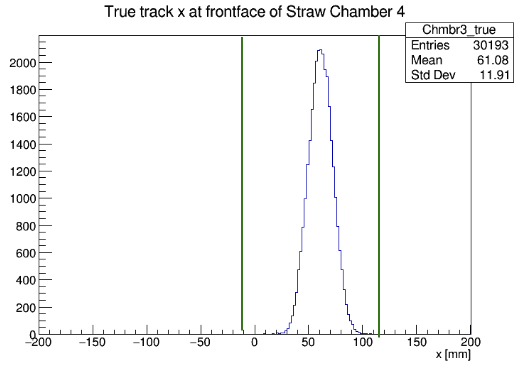
\includegraphics[width=.45\linewidth]{plots/BeamC4.png}}

            \makebox[.5\linewidth]{\small (c) Straw chamber 3}%
            \makebox[.5\linewidth]{\small (d) Straw chamber 4}%
        \end{minipage}
        \caption{Plots of current NA62 beam coordinates at each straw chamber with the beam hole walls noted by the green vertical lines}
        \label{fig:nombeam} 
    \end{figure}


    To accommodate a neutral beam, the beam holes in the Straw stations would have to become centred at 0 in the X dimension, creating a symmetric detector design. 
    However using the current NA62 beam setup it is clear the hole centred at 0 would be incompatible as from Figure \ref{fig:nombeam} the beam would impact the detector. To fix this issue the TRIM5 magnet would be removed, allowing the beam to travers along the z-axis until the interaction with the MNP33 magnetic field allowing the beam to pass through Straw chambers 1 and 2 but resulted in the beam impacting chamber 4 as shown in Figure \ref{fig:nofit}.

    \begin{figure}[H]
        \begin{minipage}{\linewidth}
          \makebox[.5\linewidth]{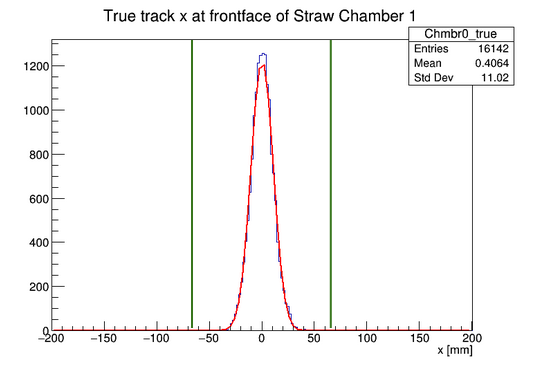
\includegraphics[width=.45\linewidth]{plots/sym1.png}}%
          \makebox[.5\linewidth]{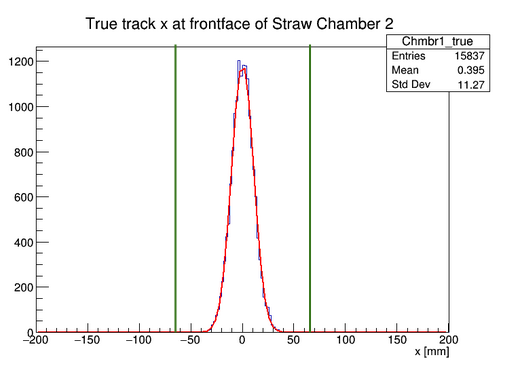
\includegraphics[width=.45\linewidth]{plots/sym2.png}}
      
          \makebox[.5\linewidth]{\small (a) Straw chamber 1}%
          \makebox[.5\linewidth]{\small (b) Straw chamber 2}%
      
          \medskip
      
          \makebox[.5\linewidth]{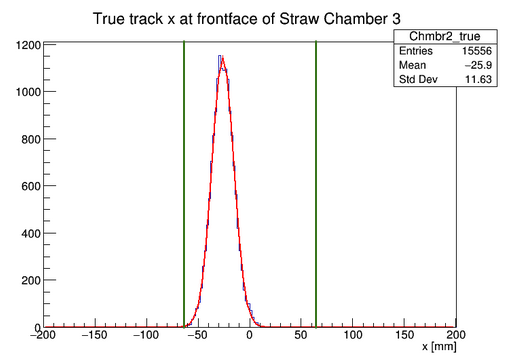
\includegraphics[width=.45\linewidth]{plots/sym3.png}}%
          \makebox[.5\linewidth]{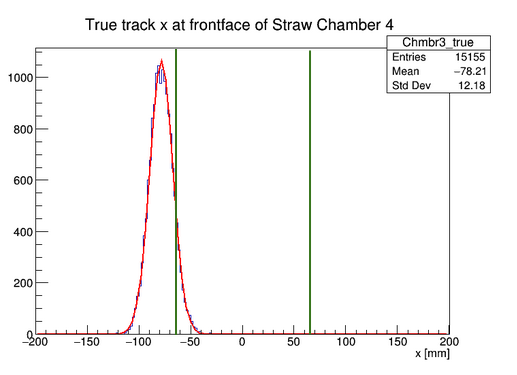
\includegraphics[width=.45\linewidth]{plots/sym4.png}}
      
          \makebox[.5\linewidth]{\small (c) Straw chamber 3}%
          \makebox[.5\linewidth]{\small (d) Straw chamber 4}%
        \end{minipage}
        \caption{Plots of symmetric straw chambers with current NA62 beam parameters}
        \label{fig:nofit}
      \end{figure}
    \section{SlimMC}



    \ifSubfilesClassLoaded{%
        \bibliographystyle{IEEEtran}
        \bibliography{../../references.bib}%
    }{} 
\end{document}